\section{Theorie}
\label{sec:Theorie}
\subsection{Grundlagen}
Linsen bestehen in der Regel aus einem Material, das optisch dichter ist als das Umgebungsmaterial. Wenn ein Lichtstrahl auf eine Linse trifft, wird er beim Eintritt und
Austritt aus dem Linsenmedium gebrochen. Es gibt zwei verschiedene Linsenarten. Die
Sammellinse wird zum Linsenrand dünner. So bündelt sie ein paralleles Licht im Brennpunkt. Die Brennweite $f$ und die Bildweite $b$ sind positiv. Es entsteht also ein reelles
Bild, das auf einem Schirm sichtbar gemacht werden kann.
\begin{figure}[H]
   \begin{center}
   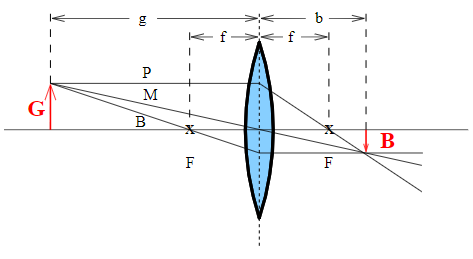
\includegraphics[width = 7.5cm, height= 4cm]{Sammellinse.png}
   \caption{Bildkontruktion zur Sammellinse.\protect\cite{AL}}
   \end{center}
   \label{fig:Sammellinse}
   \end{figure}
   \noindent
Die zweite Linsenart ist die Zerstreuungslinse. bei der die Brennweite $f$ und die Bildweite
$b$ negativ sind. Es entsteht ein virtuelles Bild.
\begin{figure}[H]
   \begin{center}
   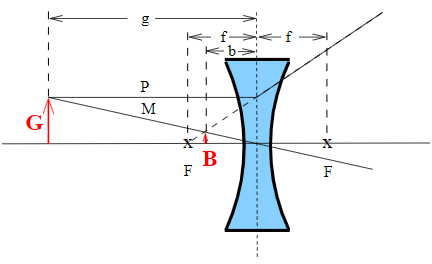
\includegraphics[width = 7.5cm, height= 4.5cm]{Zerstreuungslinse.png}
   \caption{Bildkontruktion zur Zerstreuungslinse.\protect\cite{AL}}
   \end{center}
   \label{fig:Zerstreuungslinse}
   \end{figure}
   \noindent
Bei dünnen Linsen, wie in Abbildung 1 und Abbildung 2, wird bei der Bildkonstruktion
die Brechung auf eine Mittelebene reduziert. Dies ist bei dicken Linsen, wie in Abbildung
3 dargestellt, nicht möglich.
\begin{figure}[H]
   \begin{center}
   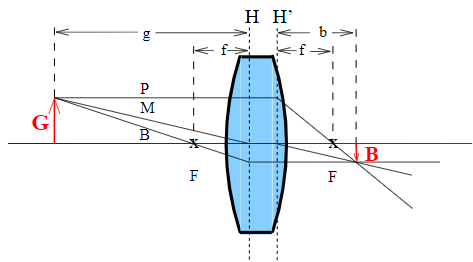
\includegraphics[width = 7cm, height= 4cm]{dicke Linsen.png}
   \caption{Bildkontruktion zur dicke Linsen.\protect\cite{AL}}
   \end{center}
   \label{fig:dicke Linsen}
   \end{figure}
   \noindent
Hierzu werden zwei Hauptebenen $H$ und $H´$
eingeführt. Es werden drei Strahlen konstruiert.\\
Der Parallelstrahl $P$ verläuft parallel zur optischen Achse, wird dann an der Mittelebene
oder Hauptebenene gebrochen und wird zum Brennpunktstrahl $B$, der durch den Brennpunkt der Linse verläuft.\\
Der Mittelpunktstahl $M$ verläuft durch die Mitte der Linse und ändert seine Richtung
nicht. Aus der geometrischen Bildkonstruktion ergibt sich folgendes Abbildungsgesetz
\begin{equation}
    V=\frac{B}{G}= \frac{b}{g}.\\
   \end{equation}
\noindent
 Dabei ist $V$ der Abbildungsmaßstab, $B$ die Bildgröße, $G$ die Gegenstandsgröße, $b$ die
   Bildweite und $g$ die Gegenstandsweite. Für dünne Linsen gilt die Linsengleichung  
   \begin{equation}
    \frac{1}{f}=\frac{1}{b}+ \frac{1}{g}.\\
   \end{equation}
\noindent
Für dicke Linsen wird die Mittelebene durch die Hauptebenen ersetzt, sodass die Brennweite, die Gegenstandsweite und die Brennweite zur jeweiligen Hauptebene bestimmt
werden, so behält die Linsengleichung ihre Gültigkeit. Jedoch gilt Gleichung (2) nur für
achsennahe Strahlen, da bei achsenfernen Strahlen das Licht stärker gebrochen wird,
sodass Abbildungsfehler entstehen und das Bild des Gegenstandes nicht mehr scharf
ist. Der Brennpunkt von achsenfernen Strahlen liegt näher an der Linse als der von
achsennahen Strahlen. Dies wird als sphärische Abberration bezeichnet. Der Brennpunkt
des blauen Lichtes liegt näher an der Linse als der vom roten Licht, da durch Dispersion
das blaue Licht stärker gebrochen wird. Das wird chromatische Abberration genannt.
Die Brechkraft wird berechnet durch
\begin{equation}
    D=\frac{1}{f}.\\
   \end{equation}
\noindent
Die Einheit der Brechkraft ist Dioptrie (1 dpt =1/m). Bei einem Linsensystem addieren
sich die Brechkräfte
\begin{equation}
    D=\sum_{i}^{N} D_i .\\
   \end{equation}
\subsection{Methode von Bessel}
Für die Bestimmung der Brennweite einer Linse nach der Methode von Bessel wird der
Abstand zwischen Gegenstand und Bild gemessen, anschließend werden zwei Positionen
der Linse gesucht, an denen ein scharfes Bild auf dem Schirm erscheint. Für diese
beiden Linsenpositionen werden dann jeweils die Bildweite $b$ und die Gegenstandsweite $g$
gemessen. Die Brennweite der Linse lässt sich dann mit Hilfe folgender Formel berechnen
\begin{equation}
 f=\frac{e^2+d^2}{4e}.\\
   \end{equation}
\noindent
Dabei ist
\begin{equation}
   e=g_1+b_1=g_2+b_2\\
      \end{equation}
   \noindent
der Abstand zwischen Gegenstand und Bild und
\begin{equation}
   d=|g_1-b_1 |= |g_2-b_2 | \\
       \end{equation}
    \noindent
der Abstand zwischen Linsenposition 1 und 2.
\begin{figure}[H]
   \begin{center}
   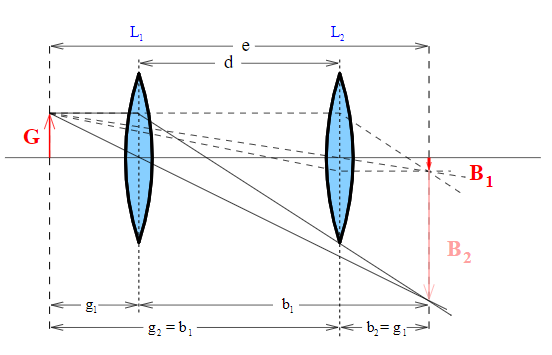
\includegraphics[width = 9cm, height= 6cm]{Bessel.png}
   \caption{Schematische Darstellung der Abstände bei der Methode von Bessel.\protect\cite{AL}}
   \end{center}
   \label{fig:Bessel}
   \end{figure}
   \noindent
\subsection{Methode von Abbe}
Bei der Bestimmung der Brennweite eines Linsensystems nach der Methode von Abbe
werden Brennweite und Lage der Hauptebenen aus dem Abbildungsmaßstab $V$ bestimmt.
Da die Gegenstandsweite und die Bildweite bei einem Linsensystem ebenso wie bei
dicken Linsen mit Hilfe von Hauptebenen bestimmt werden und diese nicht bekannt sind,
wird ein Punkt $A$ bestimmt, von dem aus die Gegenstandsweite $g´$ und die Bildweite $b´$
gemessen werden können. Für diese Weiten gelten folgende Formeln
\begin{equation}
   g´=g+h=f \Bigl(1+\frac{1}{V} \Bigr)+h\\
\end{equation}
\noindent und
\begin{equation}
b´=b+h´=f(1+V)+h´.\\
\end{equation}
\noindent
Mit Hilfe dieser Abstände und dem Abbildungsmaßstab $V$ kann die Brennweite $f$ und die
Lage der Hauptebenen bestimmt werden.
\begin{figure}[H]
   \begin{center}
   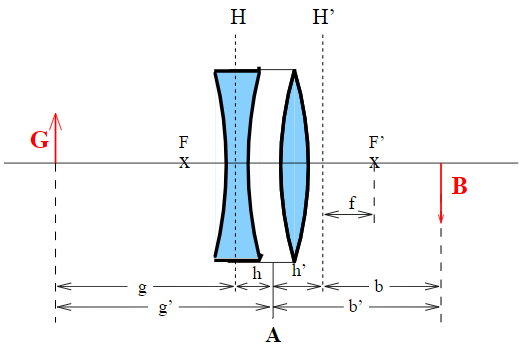
\includegraphics[width = 9cm, height= 6cm]{Abbe.png}
   \caption{Schematische Darstellung der Abstände bei der Methode von Abbe.\protect\cite{AL}}
   \end{center}
   \label{fig:Abbe}
   \end{figure}
   \noindent